\documentclass{standalone}

\usepackage[dvipsnames]{xcolor}
\usepackage{tikz}

\begin{document}

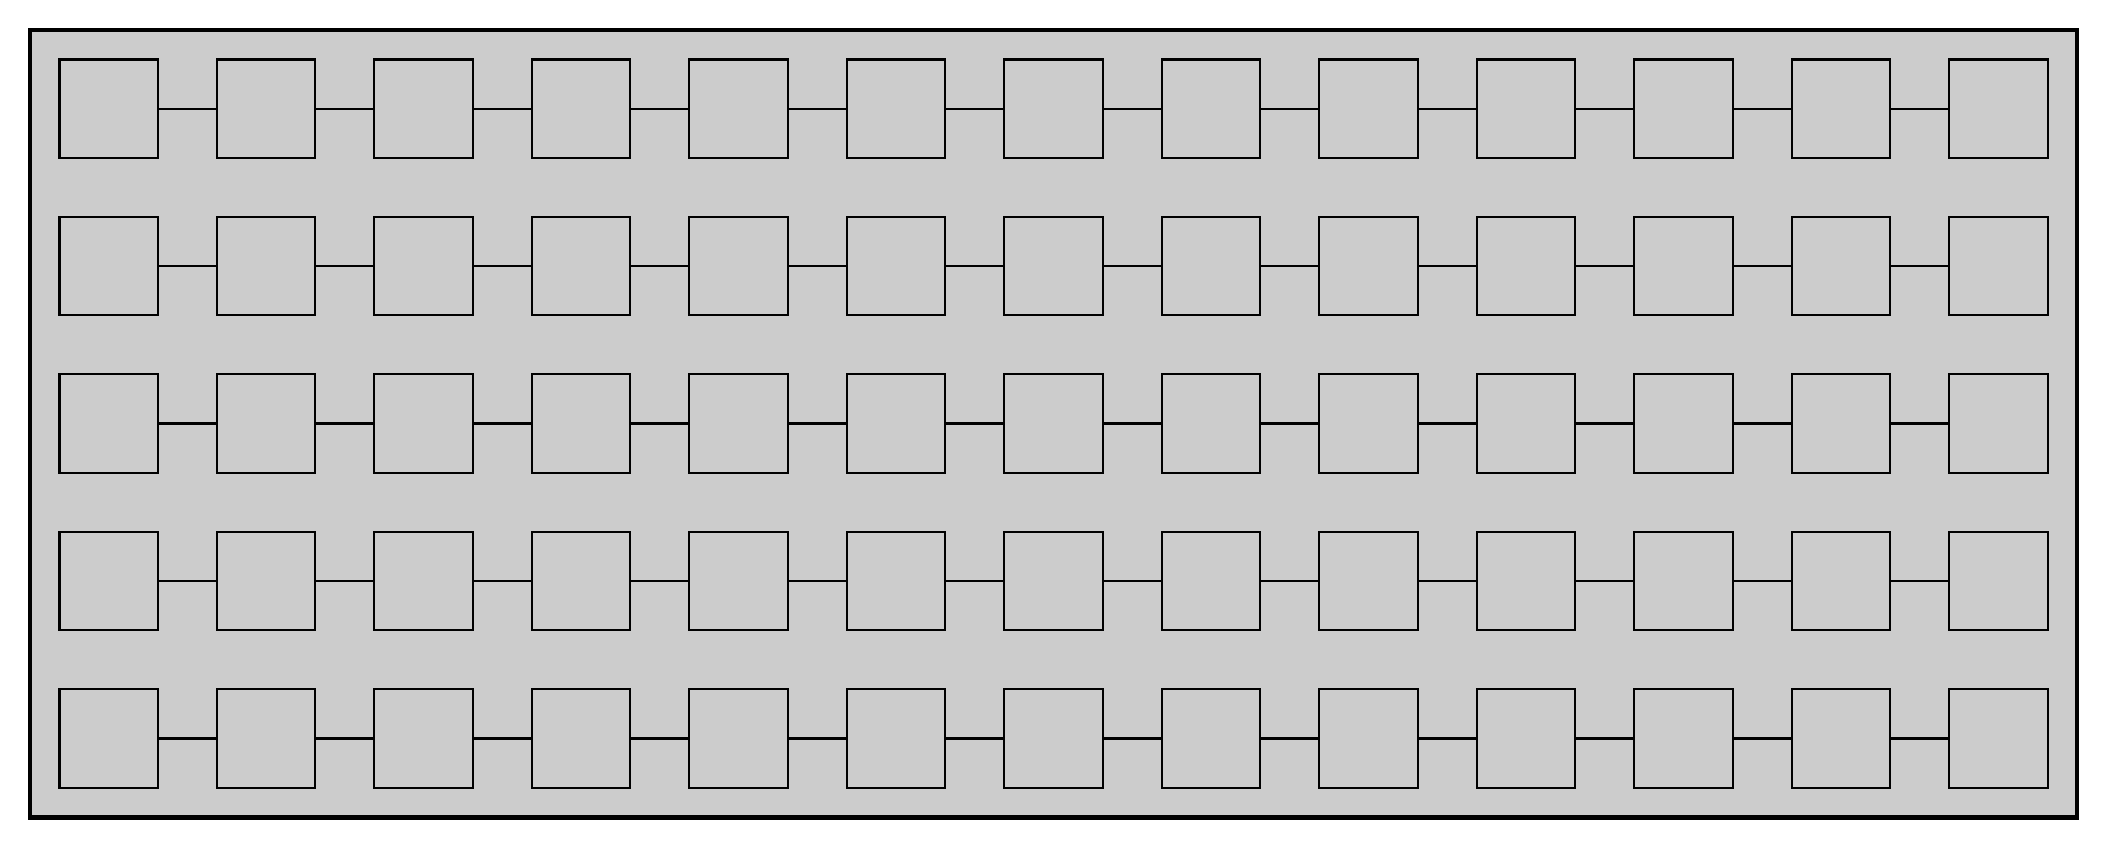
\begin{tikzpicture}
  \draw[ultra thick, fill=gray!40] (0,0) -- (0,10) -- (26,10) -- (26,0) -- cycle;

  \foreach \i in {0,1,...,12}
    \foreach \j in {0,1,2,3,4}
      \node[draw, thick, minimum size=1.25 cm] (n\i\j) at ({1+2*\i}, {1 + 2*\j}) {};
    
  \foreach \i/\ii in {0/1,1/2,2/3,3/4,4/5,5/6,6/7,7/8,8/9,9/10,10/11,11/12}
    \foreach \j in {0,1,2,3,4}
      \draw[thick] (n\i\j) -- (n\ii\j);
\end{tikzpicture}

\end{document}
